\documentclass[12pt]{article}

\usepackage[fontset=none]{ctex}
\setCJKmainfont{Noto Serif CJK SC}
\setCJKsansfont{Noto Serif CJK SC}
\setCJKmonofont{Noto Sans CJK SC}

\usepackage{graphicx,float,indentfirst,amsmath,amssymb,geometry,subfig,hyperref,tikz}

\hypersetup{hidelinks}

\geometry{a4paper,scale=0.8}

\title{偏振}
\author{}
\date{\today}

\begin{document}

\maketitle
\setlength{\parindent}{2em}

\section*{摘要}

本实验实际观察了光的偏振特性,并通过相关测量,学习了如何确定偏振片轴的方向,验证了透射光强与透射轴夹角的关系,并研究了1/4玻片,1/2玻片和全玻片的特性。

\section{观测布儒斯特角和偏振器的特性}

\subsection{原理}

将电磁波分解为两个正交的矢量P,S。P代表平行于入射面,S垂直于入射面。根据菲涅耳公式,在特定的角度,可以使P光的反射率为0,这样放射光就变成了完全线偏光。这个特定的角度就是布儒斯特角。由菲涅耳公式可知:此时$\theta_i + \theta_t = \frac{\pi}{2}$,故有$\theta_B = \arctan{n}$。

为了检验偏振光,我们必须知道偏振光通过偏振片后的光强规律,即马吕斯定律。设光场振动方向和透射轴方向成$\theta$,有:$T_{\theta} = (T_1-T_2)\cos^2{\theta}+T_2$。

\subsection{实验过程及数据分析}

首先我们测定布儒斯特角和起偏器B的透射轴夹角,我们先读出正入射时的方位角,转动平台,找到反射光能完全被偏振片消光的位置,这就是布氏角的位置,对应的起偏器角度就是透射轴在水平方向上的角度。(因为我们通过光路确保入射面水平,处于布氏角时透射轴水平能实现完全消光)为了减少误差,在扰动后重复上述过程,测量三次取平均。结果如下表:

\begin{table}[H]
    \centering
    \begin{tabular}{|c|c|}
    \hline
    开始时平台方位角          & $354^\circ 05'$ \\ \hline
    $\alpha_{B_i}$    & $P_{para_i}$    \\ \hline
    $297.5^\circ 25'$ & $89.2^\circ$    \\ \hline
    $297.5^\circ 28'$ & $89.0^\circ$   \\ \hline
    $297.5^\circ 13'$ & $89.5^\circ$    \\ \hline
    \end{tabular}
    \caption{布氏角与起偏器透射轴}
    \label{tab:A1}
\end{table}

得到平均值$\alpha_B = 297.5^\circ22'$,故而布氏角测量值$\theta_B = 56.5^\circ 17'$,折射率$n=1.532$。同时,取平均,起偏器的透射轴在水平方位的方位角为$P_{para_i}=89.23^\circ$。

进一步,来验证马吕斯定律。使用光强探测器,调整两偏振片(起偏器P和检偏器A)的夹角,在不同夹角下,测定光强$I_m$,结果如下表:

\begin{table}[H]
    \centering
    \begin{tabular}{|c|c|l|l|l|l|l|l|l|l|l|}
    \hline
    $\theta (^\circ)$ & 0.0   & 15.0  & 30.0  & 45.0  & 60.0  & 75.0  & 80.0  & 84.0  & 87.0  & 90.0  \\ \hline
    $I_m(mV)$    & 6.247 & 5.821 & 4.672 & 3.117 & 1.561 & 0.429 & 0.197 & 0.078 & 0.023 & 0.006 \\ \hline
    \end{tabular}
    \caption{马吕斯定律}
    \label{tab:A2}
\end{table}

测量中,$R=100\Omega$,偏正器P透射轴在水平方向的方位角同上。为验证马吕斯定律,将数据归一化,并做出图,如下图:

\begin{figure}[H]
    \centering
    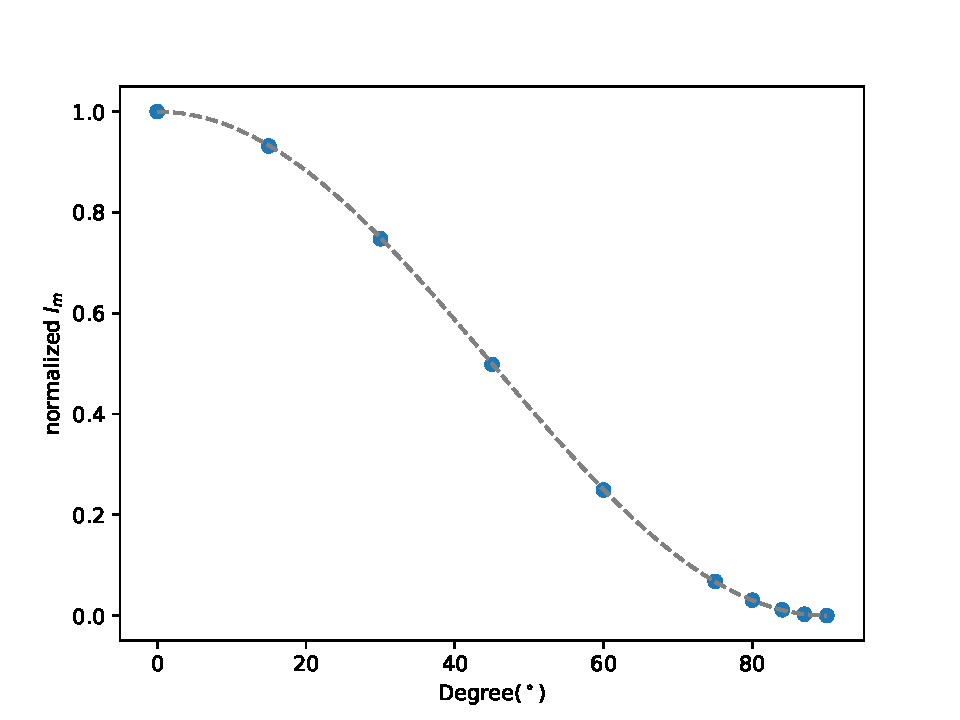
\includegraphics[width = 0.7\textwidth]{fig1.pdf}
    \caption{马吕斯定律验证}
    \label{fig:1}
\end{figure}

残差平均值为:-0.004,很接近0。图中实验所测点几乎都落在了虚线上。说明理论与实验符合良好,马吕斯定律得到了验证。

\section{波片的特性研究}

\subsection{原理}

除了常规的某个轴透光的偏振片,还有“推迟器”。其作用是利用快轴与慢轴的折射率不同,使快慢轴之间的电场产生相位差。而这一相位差又会改变偏振光的偏振态。通过测定这样的偏振态我们就可以知道待测推迟器的性质。

\subsection{实验过程及数据分析}

首先我们有两个1/4玻片,其中之一已知快轴的大致方向,我们需要知道其轴方向。将待测波片C放在已正交消光的偏振器P和A之间,旋转C,三者仍消光时,C的轴方向便平行于P的透射轴方向。这是由于对于线偏光而言,若光与轴之间有夹角,经过1/4玻片后变为圆或者椭圆偏光,无法完全消光,故保证完全消光可保证快慢轴方向与透射轴方向相同。通过光强探测器来观测消光情况,尽量调整到完全消光。偏振片P,A的配置与第一部分实验相同。最终结果如下:

$C_0$快轴在竖直方向(快轴大致沿偏振片的白点方向,由此可区分快慢轴),示数为$C_0=65.3^\circ$。$C_x$的某个轴在竖直方向时,示数为$C_x=222^\circ$。

下面探究将两个1/4玻片组合会等效得到什么。通过偏振片的矩阵表达推导可知,当两玻片轴平行或者正交的时候,要么等效于全玻片(快轴正交),要么等效于1/2玻片(快轴平行)。

先使$C_0$快轴与上面测定的$C_x$的轴平行(都在竖直方向),改变起偏器产生的偏振光的水平夹角,通过调整检偏器使其消光,得到消光时检偏器的竖直夹角,结果如下表:

\begin{table}[H]
    \centering
    \begin{tabular}{|c|c|l|l|}
    \hline
    起偏与水平夹角$\beta (^\circ)$  & 15.0 & 30.0 & 45.0 \\ \hline
    检偏与竖直夹角$\alpha (^\circ)$ & 12.5 & 27.4 & 43.2 \\ \hline
    \end{tabular}
    \caption{双1/4玻片组合1}
    \label{tab:A3}
\end{table}

在这一情况下,消光方向与竖直方向的夹角近似相当于偏振方向与水平方向的夹角。如下图:
 
\begin{figure}[H]
    \centering
    \begin{tikzpicture}[x=0.75pt,y=0.75pt,yscale=-1,xscale=1]
%uncomment if require: \path (0,300); %set diagram left start at 0, and has height of 300

%Shape: Axis 2D [id:dp9782410357926951] 
\draw  (50,153) -- (255.33,153)(155.4,58) -- (155.4,248) (248.33,148) -- (255.33,153) -- (248.33,158) (150.4,65) -- (155.4,58) -- (160.4,65)  ;
%Straight Lines [id:da06789510095583484] 
\draw    (53.33,177) -- (265.39,126.46) ;
\draw [shift={(267.33,126)}, rotate = 166.6] [color={rgb, 255:red, 0; green, 0; blue, 0 }  ][line width=0.75]    (10.93,-3.29) .. controls (6.95,-1.4) and (3.31,-0.3) .. (0,0) .. controls (3.31,0.3) and (6.95,1.4) .. (10.93,3.29)   ;
%Straight Lines [id:da3355306318932588] 
\draw    (187.33,242) -- (125.01,67.88) ;
\draw [shift={(124.33,66)}, rotate = 70.3] [color={rgb, 255:red, 0; green, 0; blue, 0 }  ][line width=0.75]    (10.93,-3.29) .. controls (6.95,-1.4) and (3.31,-0.3) .. (0,0) .. controls (3.31,0.3) and (6.95,1.4) .. (10.93,3.29)   ;

% Text Node
\draw (142,92.4) node [anchor=north west][inner sep=0.75pt]    {$\alpha $};
% Text Node
\draw (232,134.4) node [anchor=north west][inner sep=0.75pt]    {$\beta $};
% Text Node
\draw (106,43) node [anchor=north west][inner sep=0.75pt]   [align=left] {消光};
% Text Node
\draw (276,116) node [anchor=north west][inner sep=0.75pt]   [align=left] {起偏};


\end{tikzpicture}
    \caption{情况一示意图}
    \label{fig:2}
\end{figure}

消光垂直于起偏,线偏振的特性几乎不变,也就是这相当于全玻片。进一步,前述$C_x$的轴指的是其慢轴。

类似的,使$C_0$快轴与上面测定的$C_x$的轴垂直。也就是将$C_0$的快轴调整到水平方向($C_0=155.3^\circ$)。在此基础上改变起偏器产生的偏振光的水平夹角,通过调整检偏器使其消光,得到消光时检偏器的竖直夹角,结果如下表:

\begin{table}[H]
    \centering
    \begin{tabular}{|c|c|l|l|}
    \hline
    起偏与水平夹角$\beta (^\circ)$  & 15.0  & 30.0  & 45.0  \\ \hline
    检偏与竖直夹角$\alpha (^\circ)$ & 165.5 & 149.2 & 130.1 \\ \hline
    \end{tabular}
    \caption{双1/4玻片组合2}
    \label{tab:A4}
\end{table}

在这一情况下,$\alpha$与$\beta$近似互补,如下图:

\begin{figure}[H]
    \centering
    \tikzset{every picture/.style={line width=0.75pt}} %set default line width to 0.75pt        

\begin{tikzpicture}[x=0.75pt,y=0.75pt,yscale=-1,xscale=1]
%uncomment if require: \path (0,300); %set diagram left start at 0, and has height of 300

%Shape: Axis 2D [id:dp9782410357926951] 
\draw  (50,153) -- (255.33,153)(155.4,58) -- (155.4,248) (248.33,148) -- (255.33,153) -- (248.33,158) (150.4,65) -- (155.4,58) -- (160.4,65)  ;
%Straight Lines [id:da06789510095583484] 
\draw    (53.33,177) -- (265.39,126.46) ;
\draw [shift={(267.33,126)}, rotate = 166.6] [color={rgb, 255:red, 0; green, 0; blue, 0 }  ][line width=0.75]    (10.93,-3.29) .. controls (6.95,-1.4) and (3.31,-0.3) .. (0,0) .. controls (3.31,0.3) and (6.95,1.4) .. (10.93,3.29)   ;
%Straight Lines [id:da3355306318932588] 
\draw    (191.33,62) -- (120.06,244.14) ;
\draw [shift={(119.33,246)}, rotate = 291.37] [color={rgb, 255:red, 0; green, 0; blue, 0 }  ][line width=0.75]    (10.93,-3.29) .. controls (6.95,-1.4) and (3.31,-0.3) .. (0,0) .. controls (3.31,0.3) and (6.95,1.4) .. (10.93,3.29)   ;
%Curve Lines [id:da37034375276219444] 
\draw    (146.33,172) .. controls (129.33,166) and (132.33,136) .. (154.33,134) ;
%Straight Lines [id:da7344717721648077] 
\draw    (58.33,125) -- (251.33,182) ;

% Text Node
\draw (129,127.4) node [anchor=north west][inner sep=0.75pt]    {$\alpha $};
% Text Node
\draw (232,134.4) node [anchor=north west][inner sep=0.75pt]    {$\beta $};
% Text Node
\draw (78,231) node [anchor=north west][inner sep=0.75pt]   [align=left] {消光};
% Text Node
\draw (276,116) node [anchor=north west][inner sep=0.75pt]   [align=left] {起偏};
% Text Node
\draw (236,187) node [anchor=north west][inner sep=0.75pt]   [align=left] {光场};


\end{tikzpicture}

    \caption{情况二示意图}
    \label{fig:3}
\end{figure}

此时,起偏方向与消光方向近似对称。这就是半波片的效果。

综合以上,$C_x$的快轴与位置轴方向应垂直,即位于读数为$132^\circ$处。

线偏光经过1/4玻片时,会变为椭圆偏振光(圆偏光也是特殊的椭圆偏振,只是长短轴相等)。让线偏光经过$C_0$,观察其通过1/4玻片时的特性。只用一个1/4玻片,快轴置于竖直方向,起偏器和检偏器按前面的方式设置,与上面调整起偏器与检偏器的位置的做法相同,只不过要寻找检偏器的最大值(即长轴方向),得到下述结果:

\begin{table}[H]
    \centering
    \begin{tabular}{|c|c|c|c|}
    \hline
    起偏与水平夹角$\beta (^\circ)$  & 22.5  & 45.0  & 67.5  \\ \hline
    长轴与竖直夹角$\alpha (^\circ)$ & 92.9  & 72.7  & 4.0   \\ \hline
    $I_{max}(mV)$            & 4.175 & 2.433 & 2.553 \\ \hline
    $I_{min}(mV)$            & 0.583 & 2.065 & 0.505 \\ \hline
    \end{tabular}
    \caption{一个1/4玻片的情况}
    \label{tab:A5}
\end{table}

当然,为了消除误差影响,完全挡住光源时,$I_0=0.005mV$,用该数据修正$I_{min}$和$I_{max}$进行下面的计算。由上述数据,可计算玻片的相延。由理论推导知,相位差$\delta$满足$|\sin{\delta_r}|=\frac{2\sqrt{I_{min}/I_{max}}}{\sin{(2\beta)}(1+I_{min}/I_{max})}$,$delta_r$的符号有旋向和波的具体表达式($delta$加在x方向还是y方向)决定,不过对椭圆长轴方位角的计算无影响,结果如下:

$\beta = 22.5^\circ, \quad \sin{\delta_r}=0.9248, \quad \delta_r = 67.64^\circ$

$\beta = 45.0^\circ, \quad \sin{\delta_r}=0.9966, \quad \delta_r = 85.2^\circ$

$\beta = 67.5^\circ, \quad \sin{\delta_r}=1.047$,由于误差,取$\sin{\delta_r}=1.0$以进行下面的计算,$\delta_r = 90^\circ$

最后计算长轴方位角,有两种算法,一是$90^\circ-\alpha$,二是$\Psi = \frac{1}{2}\arctan{(\tan{(2\beta)} \cdot \cos(\delta))}$,计算结果如下表:

\begin{table}[H]
    \centering
    \begin{tabular}{|c|c|c|c|}
    \hline
    $\beta(^\circ)$       & 22.5   & 45.0 & 67.5 \\ \hline
    用$\alpha$计算($^\circ$) & -2.9   & 17.3 & 86   \\ \hline
    用$\delta$计算($^\circ$) & -10.41 & 45   & 90   \\ \hline
    \end{tabular}
    \caption{椭圆方位角}
    \label{tab:A6}
\end{table}

注意:在第一个结果中,由于转向规定以及超过90度带来的问题,故对最终结果取负。在$\beta=45^\circ$时,接近圆偏光,所以$\Psi$为任何值都是合理的,也可以看到较大的差距(这也是圆偏光带来的差距);针对最后结果,由于两倍的$67.5^\circ$超过了$tan$的第一个分支,故而应该取$tan$的第二个分支,得到$arctan(0)=180^\circ$。虽然存在误差,但是在可接受的范围内。

\section{讨论}

在前述实验中,所谓消光,实际上是取光强探测器的读数最小值。不同设备的消光的数值不同,有0,有正,有负。这是由于光强探测器本身就有轻微的电流,在不加负载光电流的情况下就可能出现0,正,负。而实验空间本身就有光强。种种因素叠加,便使得该读数的绝对值意义不大,真正有用的是相对值。因此确保读数最小即可认为是消光。

另外,实际偏振片是不能得到完美的线偏光的。所以在最后的实验中,即便设置为$45^\circ$我们仍能看到最大值和最小值,只不过差距较小。还是一个椭圆偏振光。

\clearpage
\appendix
\section{附录}

原始数据见下表:
\begin{figure}[H]
    \centering
    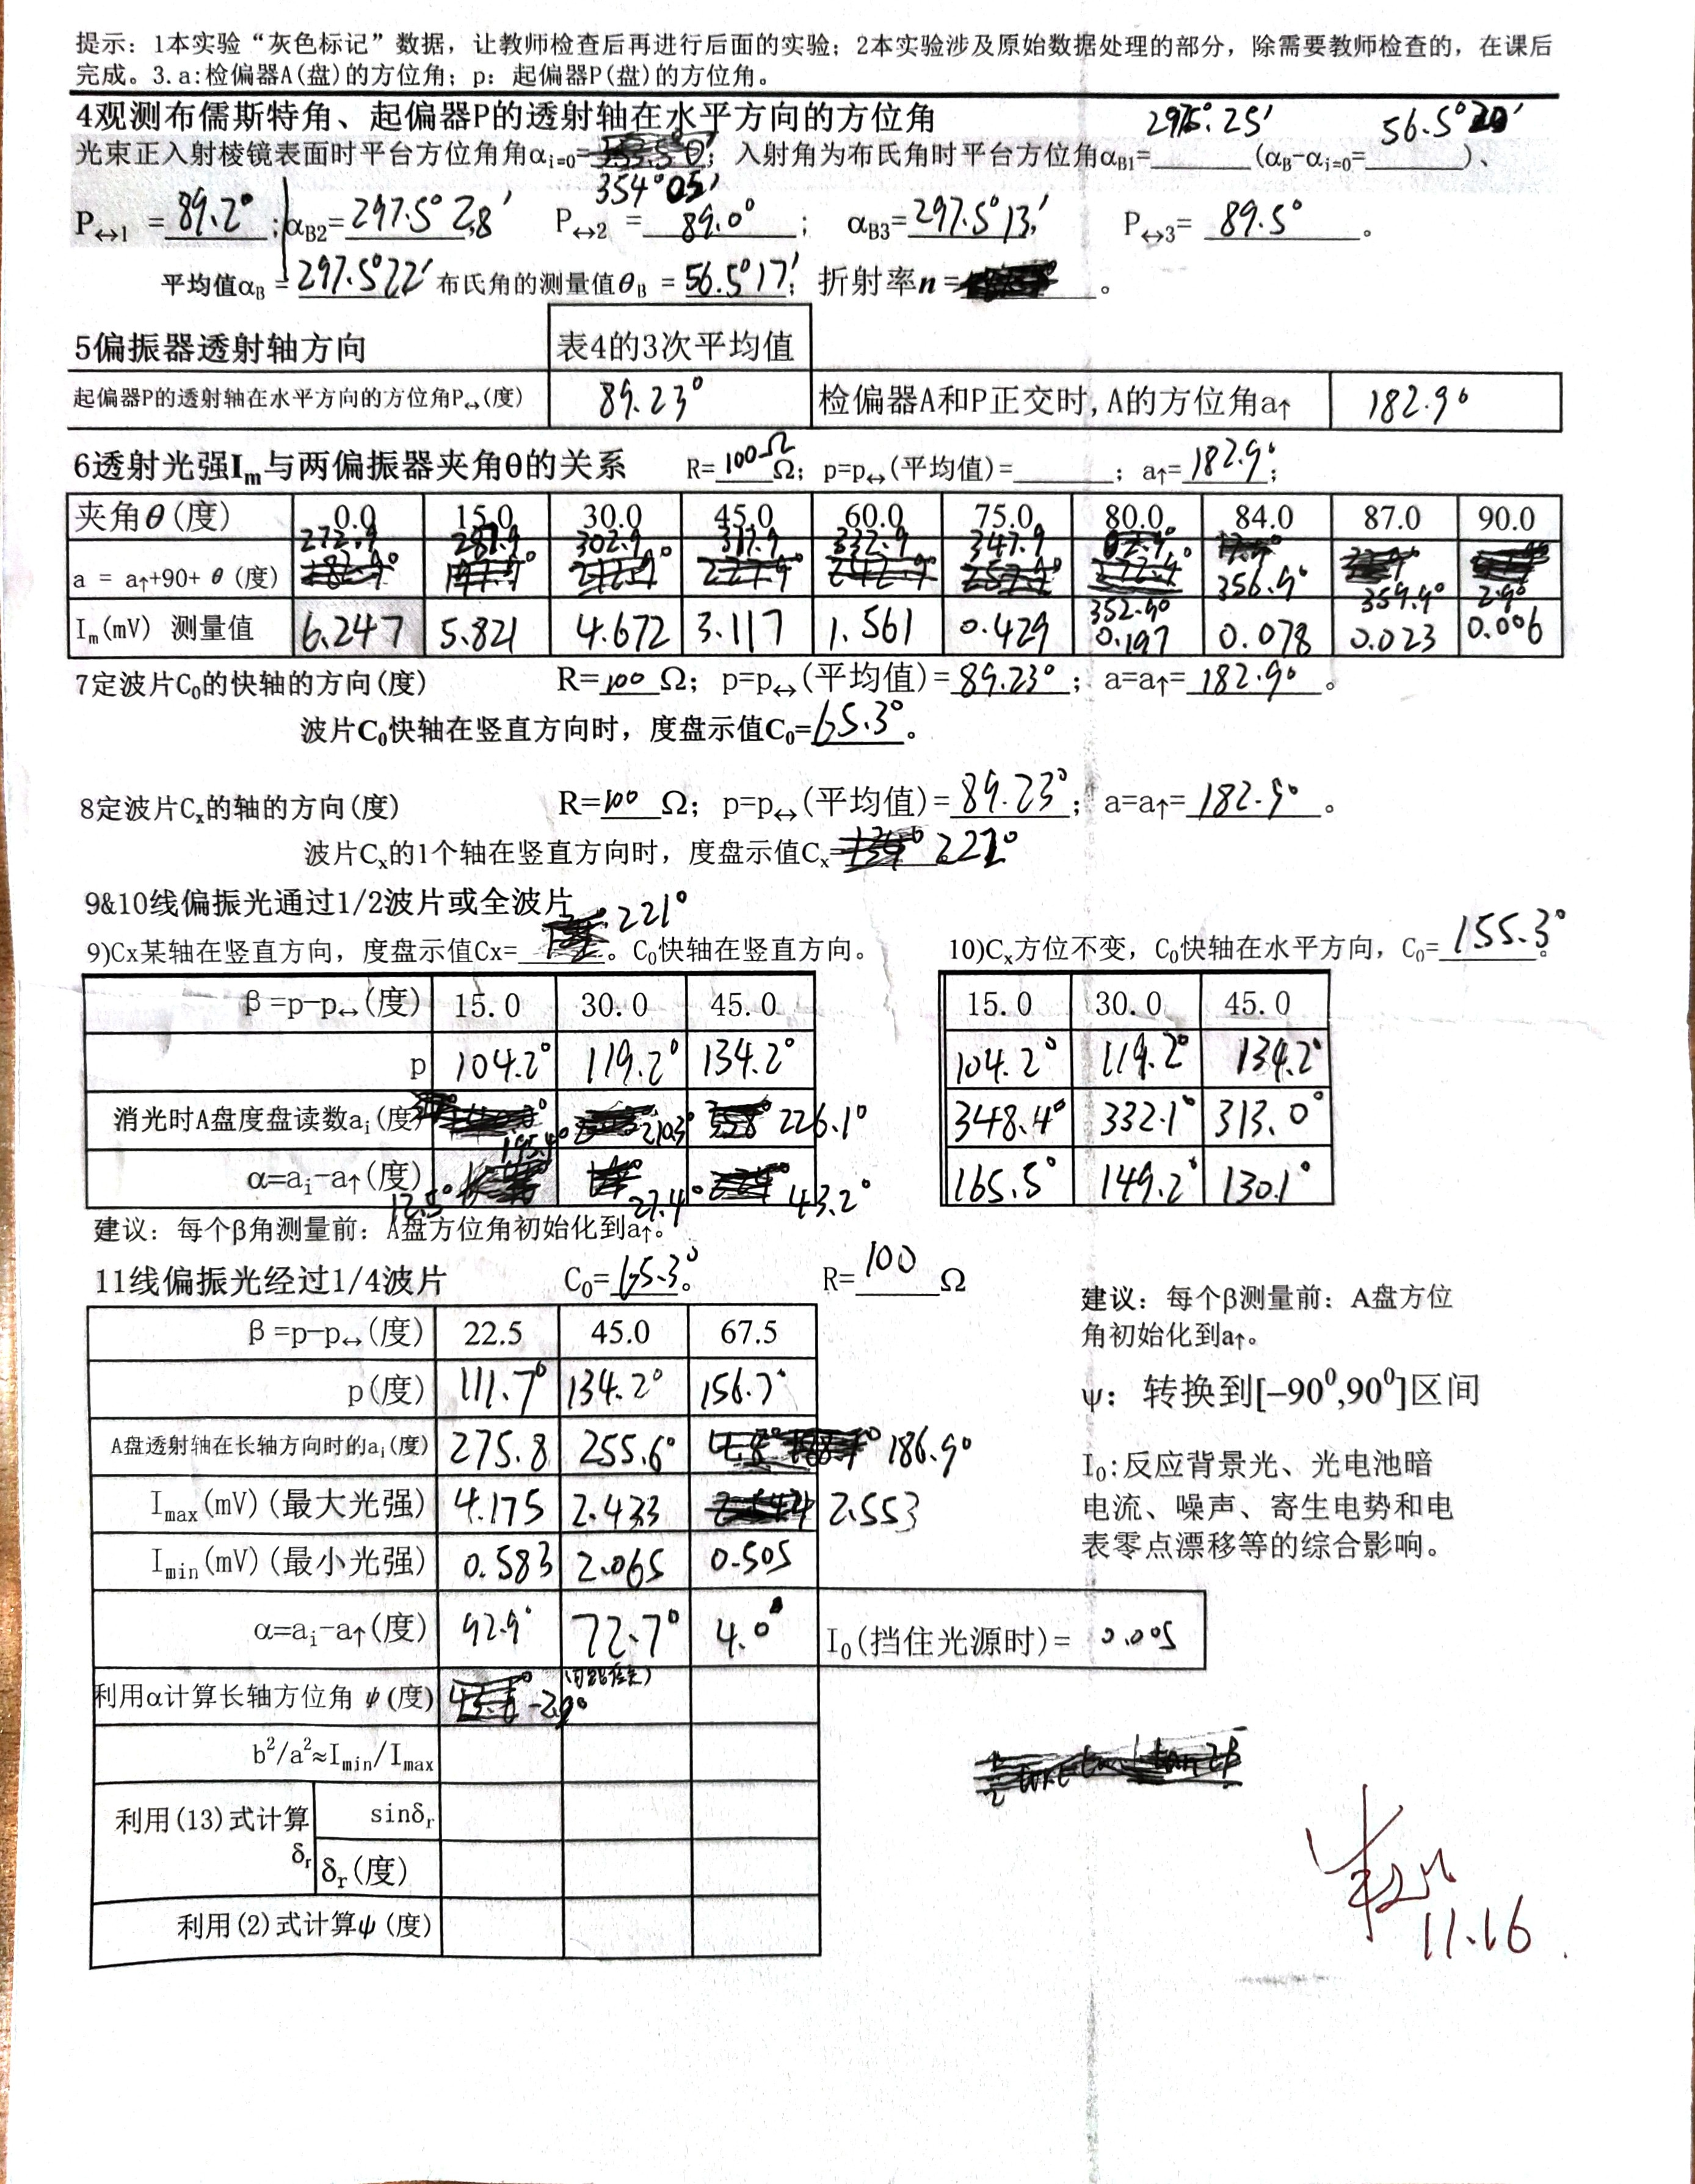
\includegraphics[width=0.9\textwidth]{IMG_20231125_125426.jpg}
\end{figure}

\end{document}
